\chapter{Introdução}
Onde, de maneira sucinta, apresenta-se:

Introdução à problemática global dentro da qual o problema específico que tratarão se enquadra; motivação e justificativa do problema e de vocês resolverem o problema (ou seja, o que precisa ser melhorado e porque algo como o que pretendem fazer o resolverá, mesmo que parcialmente); hipóteses levantadas ou argumentação principal; escopo do projeto; objetivos geral e específicos do trabalho; estrutura do documento.
Importante: Ao longo de todo o texto da monografia, quando pertinente, deve-se procurar contextualizar e explicitar em quais atividades vocês (e não as outras pessoas da equipe / empresa) atuaram / estiveram envolvidos, e o que vocês efetivamente fizeram dentro do todo apresentado.


\textbf{Importante:} Ao longo de todo o texto da monografia, quando pertinente, deve-se procurar contextualizar e explicitar em quais atividades vocês (e não as outras pessoas da equipe / empresa) atuaram / estiveram envolvidos, e o que vocês efetivamente fizeram dentro do todo apresentado.

\section{Título 2}

\subsection{Título 3}

% Introduzir Figura
\begin{figure}
	   \centering
	   		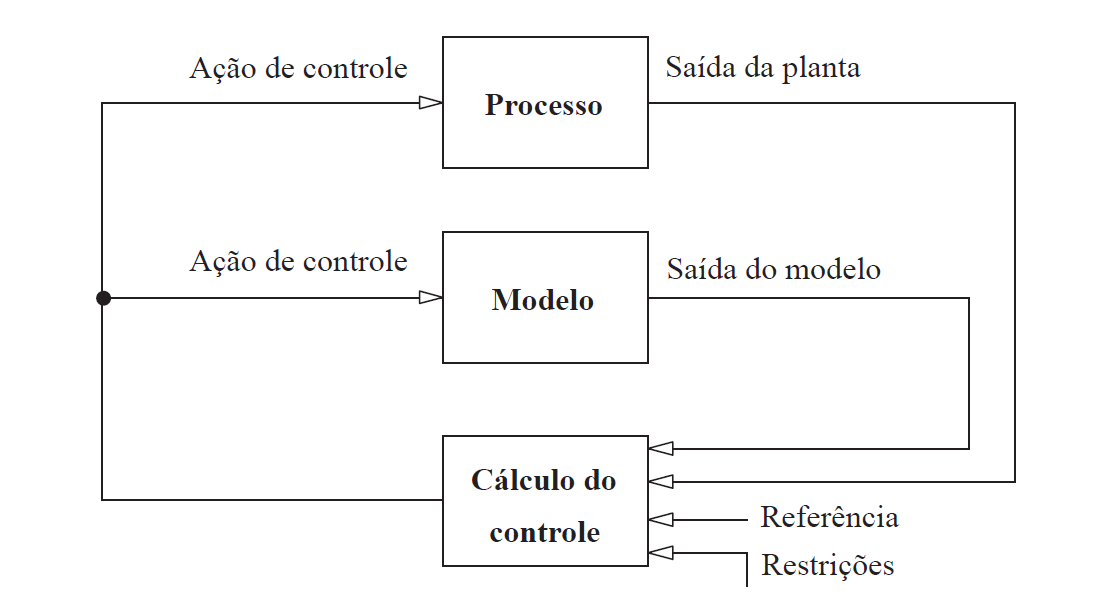
\includegraphics[scale=0.35]{figs/MPCbase.PNG} 
	   \caption{Algoritmo MPC}
	   \label{label para referencia cruzada Figura}
\end{figure}


% Lista de Item

\begin{itemize}
	\item item 1
	\item item 2
	\item item 3
\end{itemize}

% Equação
\begin{equation}
	\label{label para referencia cruzada equacoes} 
	y(t)=\sum_{i=1}^{\infty}h_i\Delta u(t-i)
\end{equation}

% Equação em linha 
$\hat{y}(t+k\mid t)= \sum^\infty_{i=1} g_i \Delta u(t+k-i\mid t)$

% Citação -  Criei o arquivo de bibliografia usando o jabref

\cite{Camacho2007} 

% Referencia Cruzada de Figura
\ref{label para referencia cruzada Figura}

% Referencia Cruzada de Equação
\ref{label para referencia cruzada equacoes}


% Tabelas

\begin{table}[h]
\begin{center}
     \caption{Índices 1 para casos factíveis}
     \begin{tabular}{| l | l | l | l |}
     \hline Índice & LP Petro & LP 2 & Diferença\\ 
     \hline $SES_y$& 60.5406 & 60.5492 & -0.0087\\
     \hline $SES_u$& 1166.1464 & 1166.1464 & 2.36*$10^{-9}$ \\
     \hline
     \end{tabular}
\label{table:indices1}
\end{center}
\end{table}